\section{Concrete Verification Methodology}

\subsection{Identity}

Identifying users will rely on
\hyperref[s:userAuth]{existing user authentication
  methodologies}.

The first option is a custom implementation; broadly
speaking, the development community (rightly) discredits
this approach.
\cite{noCustomAuth} identifies these drawbacks:

\begin{itemize}

  \item Complexity --- implementing different credentials,
        integrated into multiple
        factors, in accordance to industry-wide
        protocols/standards is difficult

  \item Risk --- data breaches will discourage new users
        and tarnish customer trust; incompatibility with
        industry standards can deter enterprise clients

\end{itemize}

Alternatively, the .NET 6 ecosystem has a comprehensive
identity platform, encompassing \enquote{users, passwords,
  profile data, roles, claims, tokens, email confirmation},
plus project templates for \gls{spa} technologies
\parencite{netIdentity}.
This is a viable solution, but it too has drawbacks: no SPA
template for Vue exists, and altering a template would be
difficult and lengthy; the components \& pages for
authentication are implemented in Razor pages alongside the
SPA, which are difficult to debug and customise.

The Auth0 \gls{identityProvider} will instead be
responsible for user authentication, outsourcing a lot of
application complexity and improving usability.
By default, Auth0 provides its own account registration \&
sign-in mechanism, but also offers external providers
(e.g., Google, LinkedIn, Twitter).
Once signed in, user data is stored on their servers,
accessed via their API.
Like .NET, an authentication process (or \enquote{flow})
for an Auth0 application can be configured for SPAs, and
they maintain Javascript packages to integrate these flows.

\paragraph{Associating Users}
% TODO check these are the right accounts
Some associations in a \gls{rdb} require the data to exist.
This presents an problem to associate users, as Auth0
stores user data separate from the application's database.

To enable such associations, the database will include
\code{User} table, storing basic user information and the
unique identifier for their user on Auth0 (see Figure
\ref{fig:auth0Data}).
This data is maintained within the
\hyperref[p:authFlow]{authentication flow}.

\begin{figure}[h]
  \centering
  \codesize
  \lstinputlisting{05 design/assets/auth0
    jwt.json}
  \caption{Auth0 User Data}
  \captiondesc{Specifically, a JWT for a new account
    created with a Github no-reply email; the \code{sub}
    field is the identifier for the user.
  }
  \label{fig:auth0Data}
\end{figure}

\paragraph{Using Social Accounts}
When users authenticate using a social provider like
Twitter, Auth0 acquires user data from the account (e.g.,
name, email, profile photo, etc.)
To ensure this basic user information is available, the
normal login mechanism using a dedicated Auth0 account will
be disabled, replaced with Google and Apple login.
Given the popularity of device requiring these accounts
(i.e., any Apple device, Gmail, Android phones), it's
highly unlikely for the average user not to have at least
one available account.

\paragraph{Authentication Flow}
\label{p:authFlow}

\begin{enumerate}

  \item An employee opens the \projectname{} website and
        clicks a button to register/log in.

  \item The page redirects to Auth0, offering social
        services with which to authenticate

  \item Once signed in, they are redirected back to the
        \projectname{} site, storing their authentication
        information in the frontend app

  \item The frontend retrieves an access token from Auth0,
        containing any user details required by
        \projectname{}

        By sending this token within API requests, employees can be
        identified and their details persisted in the database

\end{enumerate} 

\subsection{Location} 

The core of location verification is the storage of jobs
and their locations.
% TODO sequence diagram
In addition to a latitude and longitude, a job location
will also include a accuracy radius to identify the
physical size of the job site.

Using the \hyperref[ss:coordSystems]{haversine formula},
the distance between the user's current location and a job
location is measured and compared against the accuracy
radius; if their location is outside this radius, they
cannot verify their attendance at the job.

Sourcing employee's location data will use the browser's
Geolocation API, which returns their longitude and latitude
in the \gls{dd} format \parencite{geolocationApi}, as seen
in Figure \ref{fig:geolocationApi}.

\begin{figure}[h]
  \centering
  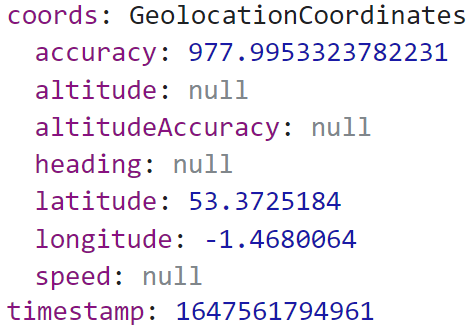
\includegraphics[width=0.5\linewidth]{05
    design/assets/geolocation api.png}
  \caption{Device location provided by the Geolocation API}
  \label{fig:geolocationApi}
  \parencite{geolocationApi}
\end{figure}

To restrict who can confirm their attendance at a job,
employees are assigned to jobs with an expected date/time
for their clock-in/out.

\subsection{Confirmation}

The implementation of the verification chain relies on a
exchange of data from the \gls{confirmee}'s device to the
\gls{confirmer}'s device.
In addition to the accountability element, the data
exchange is secured using two additional constraints to
deter employees from circumventing the mechanism.

\paragraph{Time Constraint}

Firstly, the data exchanged between the two devices will be
a time-based \hyperref[ss:otp]{one-time password}.
By applying a time constraint, it becomes harder for
\gls{conspiring-users} to share confirmation data.
Moreover, the confirmer can actively prevent this since the
process is performed in-person and it would be obvious if
an employee attempted to distribute the OTP.

\paragraph{Data Format Constraint}

Additionally, the confirmation process will exchange the
OTPs using \hyperref[ss:barcodes]{QR codes}.
Not only are they are quick \& easy to generate \& scan,
but their representation cannot be described by humans,
preventing employees from sharing the exchange data
linguistically.
Instead, the image of the QR code would need to be
transferred online using email, SMS, a messaging service,
etc., applying further pressure to the time constraint.

By using images, the user's location can also be
cross-referenced.
Modern camera/smartphones store metadata alongside the raw
pixels, known as \enquote{EXIF data} \parencite{exif},
which includes the capture date/time and geolocation.
If present in the captured image, the website can validate
this metadata as an additional control.
See Figure \ref{fig:exif} for an example.

\begin{figure}[h]
  \centering

  \begin{subfigure}{\subfigwidth}
    \centering
    \includegraphics[width=0.75\linewidth]{05
      design/assets/exif source.jpg}
    \caption{Source image}
  \end{subfigure}
  \begin{subfigure}{\subfigwidth}
    \centering
    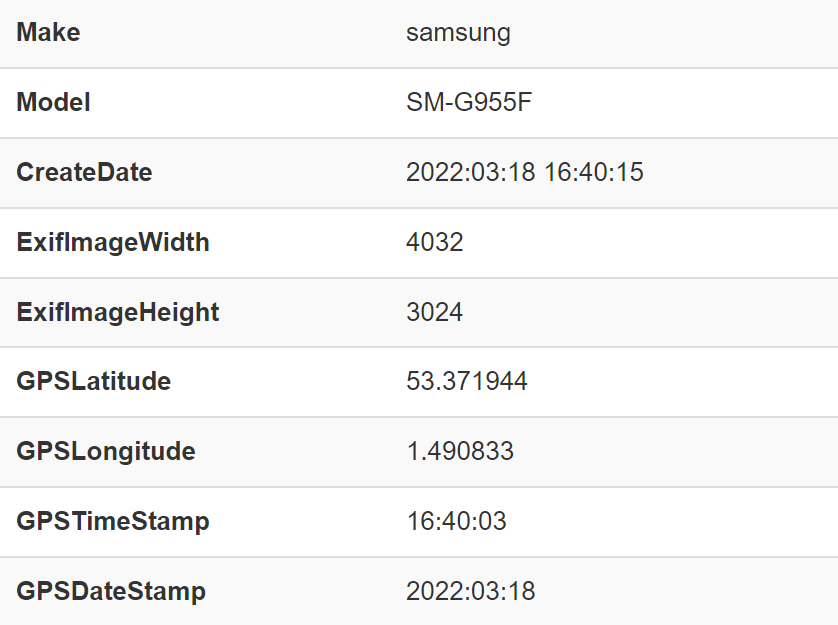
\includegraphics[width=0.75\linewidth]{05
      design/assets/exif data.png}
    \caption{Selected metadata}
  \end{subfigure}

  \caption{EXIF data}
  \label{fig:exif}
\end{figure}

\paragraph{Principle Verifier}
Drawing the from the options proposed in the
\hyperref[s:concept]{concept}, the role of principle
verifier will be assigned to the first employee to
\gls{clock-in} at a job site.
More complex approaches may be more appropriate in a
business context, but they would inherently be a business
decision which is not of concern for the scope of this
project.
